%%%%%%%%%%%%%%%%%%%% author.tex %%%%%%%%%%%%%%%%%%%%%%%%%%%%%%%%%%%
%
% sample root file for your "contribution" to a proceedings volume
%
% Use this file as a template for your own input.
%
%%%%%%%%%%%%%%%% Springer %%%%%%%%%%%%%%%%%%%%%%%%%%%%%%%%%%


\documentclass{styles/svproc}
%
% RECOMMENDED %%%%%%%%%%%%%%%%%%%%%%%%%%%%%%%%%%%%%%%%%%%%%%%%%%%
%
\usepackage{graphicx} % Required for inserting images
\usepackage{hyperref}
\graphicspath{ {./images/} }
\raggedbottom
% to typeset URLs, URIs, and DOIs
\usepackage{url}
\usepackage{tabularx}
\def\UrlFont{\rmfamily}

\begin{document}
\mainmatter              % start of a contribution
%
\title{A Network Analysis-Driven Approach to Detecting Bank Account Fraud}
%
\titlerunning{Detecting Bank Account Fraud}
%
\author{Chinmay Arvind \inst{1}(Student \#: 81088635) \and Jerry Fan\inst{2}(Student \#: 22953210),
Dmitry Kostyukov\inst{3}(Student \#: 73363350) \and Rylan Millar\inst{4}(Student \#: 33334400)}
%
\authorrunning{Chinmay Arvind et al.}
%
%%%% list of authors for the TOC (use if author list has to be modified)
\tocauthor{Chinmay Arvind , Jerry Fan, Dmitry Kostyukov, Rylan Millar}
%
\institute{University of British Columbia, Kelowna BC V1V 1V7, CAN
\\ Link to R code (data columns explained in code/code.qmd file):
\texttt{\href{https://github.com/chinmayarvind23/Bank-Account-Fraud-Detection-with-Network-Science}{GitHub Repository}}}
\maketitle              % typeset the title of the contribution
\begin{abstract}
Bank Account Fraud Detection has become increasingly important in the last few years with fraudulent entities using sophisticated methods to commit fraud, increasing the need for secure financial systems. Our paper aims to detect bank account fraud using network centrality and clustering metrics. Graph Neural Networks (GNNs), random walks, and Guilt-By-Association (GBA) methods have been used as common approaches to the problem. We created a network by connecting bank account requests (nodes) together based on the similarity of their attributes, and sampling the network's nodes. Our paper determines influential nodes in the network, an average profile for fraudulent bank account requests, fraudulent groups (fraud rings), and differences between fraudulent and non-fraudulent bank account requests. Determining influential nodes in the network tells us which nodes could be participating in fraud rings, and the average fraudulent request provides a baseline for what a fraudulent requests' attributes are which could be used for comparison with nodes that are flagged as suspicious. Determining communities in the network identifies fraud rings, and the comparison of fraudulent and non-fraudulent nodes' computed network metrics informs us on what to look for when identifying fraudulent accounts, speeding up fraud detection.
\keywords{bank fraud detection, network science, centrality, clusters}
\end{abstract}

%Introduction start
\section{Introduction}
Financial fraud is the illegal act that involves falsifying financial information to obtain funds from financial entities. Bank account fraud is a type of financial fraud where bank account information is falsified. Financial fraud is a global-scale issue that affects individuals, financial institutions, and economies resulting in major losses of funds. Our project addresses this issue by exploring bank account fraud detection from a new lens: network science. Network science is rarely used by researchers to detect financial fraud. Our study aims to pinpoint important fraudulent players, discover fraudulent groups, obtain an average fraudulent application profile, and differentiate between fraudulent and non-fraudulent applications via centrality, similarity, and clustering metrics. This novel approach will enhance our understanding of bank account fraud networks, and provide a scalable and interpretable framework for fraud detection. Our method will bridge the gap between approaches reliant on features in the bank fraud application data that set apart fraudulent and non-fraudulent requests with approaches focusing solely on network structure to detect bank account fraud.

\bigskip
\noindent\textbf{The following 4 research questions will be the focus of our paper:}

\begin{enumerate}
  \item Which were the key fraudulent players within the network?
  \item Were there any specific fraudulent groups within the network? And what were their characteristics?
  \item What was the average profile of a fraudulent customer?
  \item What differences exist between fraudulent and non-fraudulent applications?
\end{enumerate}

%Related Works start
\section{Related Works}

Rapid growth of technology in finance has made banking, credit, and other services more accessible. However, as financial systems grow, so do the risks of fraud, which threatens economic stability on a global-scale through loss of funds and trust in financial systems, therefore, understanding its history can help create more secure financial systems. Fraud has evolved from early speculative bubbles like Tulip Mania to today’s digital scams through phishing, cryptocurrency fraud, falsification of financial documents, and identity theft [4]. Fraud prevention requires robust internal security protocols to prevent data breaches, enforcement of ethical practices, and up-to-date regulations. Extracting insights on influential nodes in a network, and determining important sub-groups within a network that interact with each other frequently are two of the main goals of network analysis. Centrality metrics such as: degree centrality, betweenness centrality, closeness centrality, pagerank centrality, and eigenvector centrality are commonly used in identifying influential nodes in a network. These influential nodes are identified from the structural patterns in the network [2]. Clusters of nodes are identified as sub-groups that have high modularity (quantitative measure of durability of subgroups formed from a graph), which, in the context of bank account fraud detection can help detect fraud rings (groups of users' bank accounts working together to defraud a bank). The detection of financial fraud has been done with graph neural networks (GNNs) previously [3], where the network consists of users’ financial transactions, and is passed in its entirety to a neural network as input, where patterns in transactions are analyzed, and transactions are classified into fraudulent and non-fraudulent categories. Insurance fraud has been detected using network centrality measures, guilt-by-association (GBA) methods, random walks, GNNs, and through representation learning (where a machine learning model learns to extract insights from data automatically) [5]. Our approach will use network centrality and clustering metrics in tandem to detect if bank account requests from specific users have influence over other bank account requests in the network in terms of committing fraud, and whether these bank account requests are part of fraud rings. Bank account fraud detection has rarely been addressed from the lens of linking applications together based on the similarity of their attributes withs computed network (centrality and clustering) metrics. Wheeler et al. [7] studied various adaptive algorithms that focus on relationship analysis and pattern identification for fraud detection in financial transactions: probabilistic curve estimation based on similarity scores, best match to known cases, and density of data-based selection. One different network analysis approach for bank fraud detection is Social Network Analysis (SNA) [6], which consists of nodes representing individuals and edges representing linkages between individuals in the form of communications. In such a network, centrality metrics prove useful in identifying influential players in the network and in uncovering fraudulent activity in rings. Limitations of this fraud detection method are data collection being time-intensive to find links between individuals, and little to no means of assessing potentially fraudulent activity of individuals with no links. Our method of assessing fraudulent activity with users' bank account application alongside network metrics may prove beneficial in overcoming the above-mentioned limitations. 

%Research Design and Methodology start
\section{Methodology}

\subsection*{Research Design, Data Pipeline \& Feature Extraction}
Nodes in our network represent individuals' bank account applications, and edges exist between nodes to represent whether or not two applications had a similar value for an attribute, creating a complex undirected multigraph. The network was created as such to ensure that transactions that were similar to each other would be linked to one another, and could be used in further investigation on nodes that were deemed suspicious. The dataset for this study comprises bank account application records with fraud indicators sourced from a Kaggle dataset (cited below). Each account was labeled as fraudulent or non-fraudulent using a binary variable ’fraud\_bool’. The records in the dataset were preprocessed by removing records with missing fields to ensure that the remaining records give a complete picture of all features in the data when analyzing the nodes, and columns that did not explain a large amount of variation in the dataset were removed as part of feature selection using Principal Component Analysis (PCA). Running the entire dataset would be infeasible in a local RStudio environment due to the lengthy computation time of our edge-generating function. Therefore, we propose a sampling approach that draws a representative sample of the dataset to generate visualizations of the network. We will keep our sample sizes in the 100 to 2000 range out of a total of 743169 nodes in the dataset. The percentage of fraudulent nodes in the full data set is approximately 1\%. To ensure this proportion is consistent in our samples we will use a stratified sampling approach that takes 1\% of the data from a strata of only fraudulent nodes and the other 99\% of the data from a strata of only non-fraudulent nodes to construct the sample. We ensure that the sample is representative of the entire data set by applying the Chi-Squared test, that determines if there is a statistically significant difference between values in the columns of the sample and the full data set. The Chi-Squared test generates p-values for each column in a sample and after conducting the test on a given sample we found that samples drawn are sufficiently representative of the entire data set (p greater than 0.05), with a p-value of less than 0.05 indicating a significant difference between the sample and the entire data set for that particular column. 

\subsection*{Research Question 1: Key Fraudulent Players Within the Network}
To find the key fraudulent players within the network, we carried out a centrality-based analysis of the nodes in the sample. The sample size was 100 nodes. The centrality metrics that were computed were: eigenvector centrality, and betweenness centrality. The eigenvector and betweenness centrality scores were computed for all nodes in the sample and imputed into the sample data as new columns. The nodes were then ordered by descending centrality scores to find the most influential nodes in the network. Eigenvector centrality in the context of this research question defines the most important nodes in the network by taking into account both the quantity and quality of nodes (more important nodes a node is linked to, the higher the eigenvector centrality score), whereas betweenness centrality defines the most important nodes in terms of nodes' abilities to act as middlemen for information flow. Katz centrality was not used as a metric as its main use case is the scenario when there are nodes with an in-degree of 0, which is a rare occurrence in our multigraph. Closeness centrality was not used as a metric as it emphasizes the velocity at which information travels from one node to others, which is not relevant to our goal of finding bank account fraud occurrences as the edges connect applications that are similar. Degree centrality is too simple of a metric to capture patterns in the network structure, and was omitted from usage. PageRank centrality does not provide much more information than eigenvector centrality for an undirected network, and was also not used as a metric. Both eigenvector and betweenness centrality are used in tandem to flag nodes as suspicious and in need of further investigation in the scenario that their `fraud\_bool` column values were 0 (non-fraudulent application).

\subsection*{Research Question 2: Average Profile of a Fraudulent Account}
To get the average profile of a typical fraudulent node, we calculate the mean of numeric attributes and the mode of binary or categorical attributes for fraudulent nodes in the dataset. We then use this aggregated profile to create a new node called the typical fraud Node and add it to the dataset. Next, we compute two similarity measures -- Cosine similarity and Jaccard similarity between the typical fraud Node and all other fraudulent nodes. If the similarity score between the Typical Fraud Node and another node exceeds a predefined threshold, we draw an edge between the two nodes in the graph. The maximum number of edges possible in this graph is n-1, where n represents the total number of nodes since, in theory, each node could be connected to the typical fraud node. Comparing this theoretical maximum against the number of edges in the graph can better indicate the typical fraud node's appropriateness as an indicator for fraudulent behaviour. If the network density is high, we can see that the typical fraud node is a reliable indicator for fraudulent nodes, and this approach can be extended to evaluate new applications. By calculating the similarity score between the typical fraud node and an unknown node, we can flag the transaction as potentially fraudulent if the score is above a threshold.

\subsection*{Research Question 3: Identifying Potential Fraudulent Groups}
In order to identify groups potentially committing fraudulent activities, we use an approach involving community detection algorithms. We start by determining the average profile of a fraudulent account, creating a baseline profile for comparison. We then use the Louvain community detection algorithm which clusters nodes in a network that are more closely connected to each other than to the remaining nodes of the network. For each community, we calculated the average profile of its nodes by aggregating the attributes used to define the fraudulent profile. Next, we compare the average profile of the fraudulent accounts with the average profiles of the nodes from the four communities, allowing us to identify whether any of the communities exhibited patterns or characteristics similar to those of fraudulent accounts. Finally, we calculate the modularity of the Louvain communities, which measures how well-defined the communities are (higher values indicate meaningful clusters) to evaluate the quality of the groupings. 

\subsection*{Research Question 4: Differences Between Fraudulent and Non-fraudulent Accounts}
To explore the differences between key metrics for fraudulent and legitimate nodes within our network, the means of several network metrics are compared for both fraudulent and legitimate nodes. The utilized metrics are degree centrality, eigenvector centrality, closeness centrality, betweenness centrality, local clustering coefficient and the Jaccard coefficient. The mean degree and eigenvector centralities will provide insight into the connectivity of the two groups. Since the edges of the graph represent shared attributes amongst applicants, a significantly different eigenvector centrality or mean degree value between the two groups will signify a differences in connectivity and similarity between the two groups. The eigenvector centrality is considered because it will also take into account the proximity to important nodes. A significant difference in the closeness centrality may indicate that one group is more difficult to reach. The betweenness centrality will measure the average number of shortest paths that pass through fraudulent and legitimate nodes. This refers to the positioning of the two groups within the network and will show if one group is more central in terms of direct routes between any two nodes. The local clustering coefficient will measure the extent to which nodes form cliques with their neighbours. This will allow us to observe the difference in the presence of structural holes for fraudulent and legitimate nodes. The Jaccard Similarity provides insight into the similarities between nodes based on shared neighbours. A discrepancy in the average Jaccard similarity will suggest a difference in structural equivalence between fraudulent and legitimate nodes. The metrics are collected for 10 separate samples of 1000 nodes each of the entire dataset using stratified sampling. The metrics for these samples are averaged to remove sampling bias.

%Results start
\section{Results}

\subsection{Analyzing Key Fraudulent Accounts}

The threshold to define nodes as suspicious (influential) in the context of bank account fraud are the nodes that rank above the 75th percentile for the eigenvector centrality and betweenness centrality scores individually. For the sample of nodes that we used, we first detected the 10 most influential nodes from the top 25 percentiles of nodes having very high eigenvector centrality:

\noindent
\begin{tabular}{ | m{2cm} | m{1.5cm}| m{1.2cm}| m{1.2cm}| m{1.2cm}| m{1.1cm}| m{1.2cm}| m{2.1cm}|} 
  \hline
  \textbf{node\_id} & \textbf{payment type} & \textbf{keep alive session} & \textbf{foreign request} &  \textbf{email is free} & \textbf{fraud bool} & \textbf{bank branch count 8w} & \textbf{eigenvector centrality score}\\ 
  \hline
   10295 & 2 & 1 & 0 & 0 & 0 & 1 & 1.0000000\\ 
  \hline
  582493 & 1 & 1 & 0 & 1 & 0 & 1 & 0.9781452\\ 
  \hline
  191649 & 2 & 1 & 0 & 1 & 0 & 1 & 0.970140\\
  \hline
  132333 & 1 & 1 & 0 & 1 & 0 & 1 & 0.9595332\\
  \hline
  638068 & 1 & 1 & 0 & 0 & 0 & 1 & 0.9593648\\
  \hline
  515970 & 2 & 1 & 0 & 1 & 0 & 1 & 0.9559428\\
  \hline
  127176 & 2 & 1 & 0 & 1 & 0 & 1 & 0.9533932\\
  \hline
  288461 & 2 & 1 & 0 & 0 & 0 & 1 & 0.9517984\\
  \hline
  661285 & 1 & 1 & 0 & 0 & 0 & 1 & 0.9456791\\
  \hline
  487929 & 2 & 1 & 0 & 0 & 0 & 1 & 0.9378288\\
  \hline
\end{tabular}

\noindent{\small\textbf{Fig. 1. Table displaying the profile of the top 10 nodes with the highest eigenvector centrality.}}

\noindent We then detected the 10 most influential nodes from the top 25 percentiles of nodes with high betweenness centrality, which were:

\noindent
\begin{tabular}{ | m{2cm} | m{1.5cm}| m{1.2cm}| m{1.2cm}| m{1.2cm}| m{1.1cm}| m{1.2cm}| m{2.1cm}|} 
  \hline
  \textbf{node\_id} & \textbf{payment type} & \textbf{keep alive session} & \textbf{foreign request} &  \textbf{email is free} & \textbf{fraud bool} & \textbf{bank branch count 8w} & \textbf{betweenness centrality score}\\ 
  \hline
   512662 & 2 & 1 & 0 & 1 & 0 & 1 & 2.338539\\ 
  \hline
  10295 & 2 & 1 & 0 & 0 & 0 & 1 & 2.260064\\ 
  \hline
  127176 & 2 & 1 & 0 & 1 & 0 & 1 & 2.161004\\
  \hline
  677418 & 2 & 0 & 0 & 1 & 0 & 1 & 2.009444\\
  \hline
  132333 & 1 & 1 & 0 & 1 & 0 & 1 & 1.973075\\
  \hline
  7320322 & 2 & 0 & 0 & 1 & 0 & 1 & 1.855374\\
  \hline
  582493 & 1 & 1 & 0 & 1 & 0 & 1 & 1.830061\\
  \hline
  395008 & 2 & 1 & 0 & 0 & 0 & 1 & 1.814628\\
  \hline
  596042 & 2 & 1 & 0 & 0 & 0 & 1 & 1.812014\\
  \hline
  487357 & 2 & 0 & 0 & 1 & 0 & 1 & 1.809334\\
  \hline
\end{tabular}

\noindent{\small\textbf{Fig. 2. Table displaying the profile of the top 10 nodes with the highest betweenness centrality.}}

\noindent These detected nodes were then pooled together to create a venn diagram to find the nodes that consistently ranked high amongst both centrality metrics. The venn diagram generated was as follows:

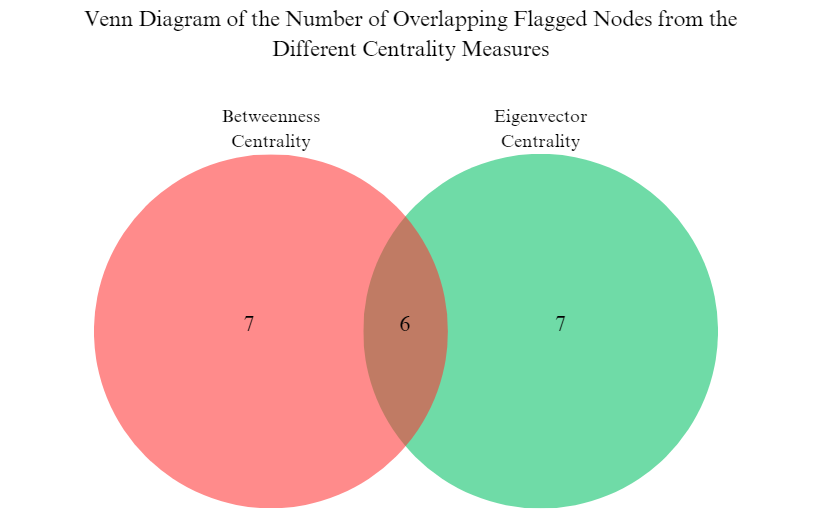
\includegraphics[scale=0.39]{venn}

\noindent{\small\textbf{Fig. 3.  The red circle represents the number of flagged nodes with high betweenness centrality, and the purple circle represents the number of flagged nodes with high eigenvector centrality, and the intersection is the number of nodes with high centralities for both metrics.}}

\smallskip
\noindent 19 nodes were flagged as having high values for both centrality metrics from the top 50 suspicious nodes from both centrality metrics. Therefore, the most influential nodes in the network according to both centrality metrics were the nodes with the following IDs: 512662, 10295, 127176, 677418, 132333, 730322, 582493, 395008, 487357, 665754, 638068, 429872, 515970, 487929, 475976, 191649, 661285, 377963, and 714113. \textbf{Note: The results from this research question could be different if a new graph is created due to the sample of nodes being random}

\subsection{Obtaining the Average Profile of a Fraudulent Account}
\normalfont
The average profile of a fraudulent account is as follows:

\begin{tabular}{ | m{7cm} | m{3cm}|} 
  \hline
  \textbf{Attribute} & \textbf{Value} \\ 
  \hline
  payment\_type & 2 \\ 
  \hline
  keep\_alive\_session & 0 \\ 
  \hline
  foreign\_request & 0 \\
  \hline
  email\_is\_free & 1 \\
  \hline
  bank\_branch\_count\_8w & 210.1815 \\
  \hline
  zip\_count\_4w & 1648.506 \\
  \hline
  name\_email\_similarity & 0.3859064 \\
  \hline
  bank\_months\_count & 17.3637 \\
  \hline
  housing\_status & 1 \\
  \hline
  velocity\_6h & 5251.171 \\
  \hline
  phone\_home\_valid & 0 \\
  \hline
  current\_address\_months\_count & 30 \\
  \hline
\end{tabular}

\noindent{\small\textbf{Fig. 4. Table representing the average profile of a fraudulent account based on the attributes of our dataset.}}

\noindent Utilizing the average fraudulent node, we set thresholds for jaccard similarity and cosine similarity calculations. The thresholds for the similarity calculations were determined based on the characteristics of the dataset and balance between meaningful detection and noise reduction. If the similarity score was above the threshold, then an edge was be drawn between the typical fraud node and the actual node. A threshold of 0.5 was chosen for Jaccard similarity, meaning that at least 50\% of features, whether binary or numeric, needed to match; numeric features were considered to match if their difference was within a tolerance of 0.1, ensuring a focus on significant feature overlap. In the case of Cosine similarity, a stricter threshold of 0.7 was considered to capture strong alignment in feature vectors, considering both binary and numeric data. While Jaccard coefficient emphasizes exact matching at the feature level, Cosine similarity captures more general structural alignment. Together, these thresholds were validated to effectively highlight fraudulent connections in the network while mitigating excessive noise. \textbf{The maximum possible edges are: 6877.}

\smallskip
\noindent
\begin{tabular}{ | m{5cm} | m{2.5cm}| m{3.2cm}|}
  \hline
  \textbf{Metric} & \textbf{Value} & \textbf{Percentage}\\ 
  \hline
  \textbf{Number of Jaccard Edges} & 0 & 0.00\%\\ 
  \hline
  \textbf{Number of Cosine Edges} & 148 & 2.15\%\\ 
  \hline
\end{tabular}

\smallskip
\noindent{\small\textbf{Fig. 5. The graph analysis indicates that the Jaccard similarity graph, with a maximum of 6877 possible edges, has 0 edges, which is 0.00\% of the total possible connections. On the other hand, the Cosine similarity graph contains 148 edges, accounting for only 2.15\% of the maximum possible edges.}}

\subsection{Identifying Potential Fraudulent Groups}
After visualizing the graph, we applied the Louvain method for community detection to group the nodes into clusters. The resulting graph is shown below.

\begin{center}
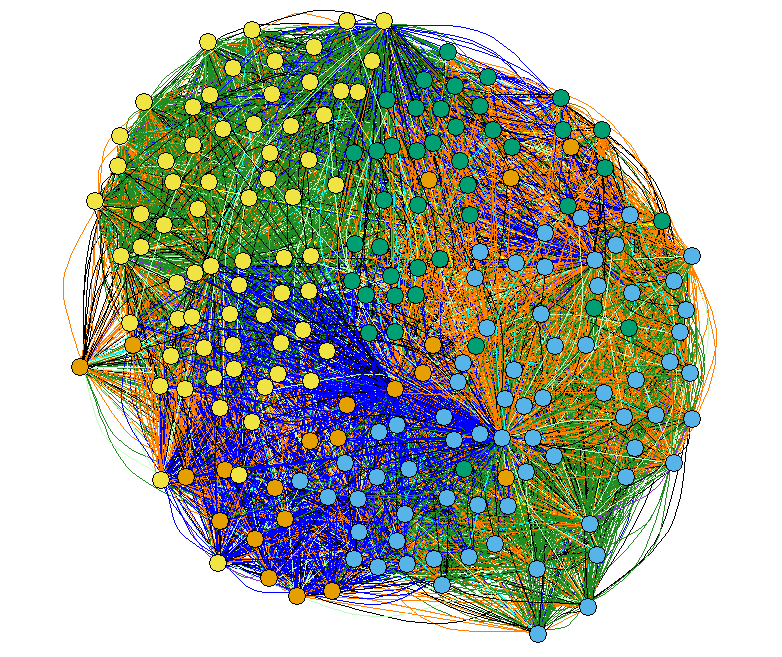
\includegraphics[scale=0.43]{q2comm}  
\end{center}
\noindent{\small\textbf{Fig. 6. The above graph was created from a sample size of 200 nodes. The colors of the nodes represent the 4 communities identified.}}

\bigskip
\noindent The table below summarizes the average profiles and key statistics of the four communities detected, highlighting patterns and potential links to the characteristics of fraudulent nodes.

\bigskip
\noindent
\begin{tabular}{ | m{4.7cm} | m{1.8cm}| m{1.25cm}| m{1.25cm}| m{1.25cm}| m{1.25cm}|} 
  \hline
  \textbf{Attribute} & \textbf{Avg. Fraud} & \textbf{C1} & \textbf{C2} & \textbf{C3} & \textbf{C4}\\ 
  \hline
  payment\_type & 2 & 2 & 2 & 3 & 2 \\ 
  \hline
  keep\_alive\_session & 0 & 1 & 1 & 1 & 0 \\ 
  \hline
  foreign\_request & 0 & 0 & 0 & 0 & 0 \\
  \hline
  email\_is\_free & 1 & 1 & 1 & 1 & 1 \\
  \hline
  bank\_branch\_count\_8w & 210.18 & 234.92 & 234.92 & 100.17 & 183.48 \\
  \hline
  zip\_count\_4w & 1648.51 & 1614.70 & 1574.50 & 1500.80 & 1458.9 \\
  \hline
  name\_email\_similarity & 0.386 & 0.485 & 0.485 & 0.490 & 0.0215 \\
  \hline
  bank\_months\_count & 17.36 & 15.89 & 12.62 & 14.66 & 18.04 \\
  \hline
  housing\_status & 1 & 3 & 3 & 1 & 2 \\
  \hline
  velocity\_6h & 5251.171 & 5858.81 & 5165.11 & 5106.61 & 5235.64 \\
  \hline
  phone\_home\_valid & 0 & 0 & 0 & 0 & 0 \\
  \hline
  current\_address\_months\_count & 30 & 98 & 82 & 141 & 120 \\
  \hline
\end{tabular}

\bigskip
\noindent{\small\textbf{Fig. 7. The table above shows the average profile of a fraudulent account, derived from the attributes in our dataset alongside average profiles of the four communities identified through the Louvain community analysis.}}

\subsection{Finding Differences Between Fraudulent and Non-fraudulent Accounts}

\smallskip
\begin{tabular}{ | m{1.55cm} | m{1.65cm}| m{1.65cm}| m{1.65cm}| m{1.65cm}| m{1.65cm}| m{1.65cm}|}
  \hline
  \textbf{Metrics} & \textbf{Degree (Legit)} & \textbf{Degree (Fraud)} & \textbf{Eigen (L)} & \textbf{Eigen (F)} & \textbf{Jaccard (L)} & \textbf{Jaccard (F)}\\ 
  \hline
  \textbf{Mean} & 1380.840 & 1182.438 & 0.649 & 0.556 & 0.701 & 0.658\\ 
  \hline
\end{tabular}

\bigskip
\noindent{\small\textbf{Fig. 8. Mean Degree Centrality, Eigenvector Centrality and Jaccard Similarity of fraud accounts (F) and legitimate accounts (L).}}

\smallskip
\noindent
\begin{tabular}{ | m{1.55cm} | m{1.7cm}| m{1.7cm}| m{1.6cm}| m{1.6cm}| m{1.7cm}| m{1.7cm}|}
\hline
\textbf{Metrics} & \textbf{Closeness (Legit)} & \textbf{Closeness (Fraud)} & \textbf{Between (L)} & \textbf{Between (F)} & \textbf{Local Cluster (L)} & \textbf{Local Cluster (F)}\\ 
\hline
\textbf{Mean} & 1380.840 & 1182.438 & 0.649 & 0.556 & 0.701 & 0.658\\ 
\hline
\end{tabular}

\bigskip
\noindent{\small\textbf{Fig. 9. Mean Closeness Centrality, Betweenness Centrality and Local Clustering Coefficient of fraud accounts (F) and legitimate accounts (L).}}

\bigskip
\noindent The most substantial discrepancy between means is between the Betweenness centralities, with a difference of 42.02\%, with legitimate nodes on average having much higher betweenness centrality. This is followed by the degree centrality means and eigenvector centrality means, which on average have differences of about 16.78\% and 16.72\%, respectively. Both the degree and eigenvector centralities are higher for Legitimate nodes. Legitimate nodes have a higher Jaccard centrality with a mean difference of 6.50\%. Closeness centrality and clustering centrality have the lowest mean differences with 2.94\% and 1.31\% respectively, which are likely too small to be considered substantial.

%Discussion start
\section{Discussion}

\subsection{Key Fraudulent Accounts}
The top 25 percentiles for each centrality measure were chosen as a threshold to focus investigations onto nodes with abnormally high centrality values. The nodes that were flagged as suspicious may not themselves be fraudulent but are flagged based on their connections to other suspicious nodes with high centrality scores. The flagged nodes can be provided to domain experts as leads for a deep-dive investigation to see if any of the flagged applications were fraudulent through examining other attributes that were not a part of the dataset alongside attributes in the dataset. The flagged nodes with high centralities for both metrics should be the first nodes to be examined to see if they were part of any fraud rings as a member or as a leader. The nodes with high betweenness centrality could be involved in fraud rings as middlemen as a bank account request could be similar to many other account requests, the node with high betweenness centrality could provide the link between different account requests within a fraud ring, speeding up fraud detection with targeted node suggestions that can be investigated. Using these centrality metrics should be done as one facet of the investigative process alongside other algorithmic approaches to prevent classifying nodes falsely as fraudulent. If data from transactions within these bank accounts that were being assessed for fraud were present, it would have helped in zeroing in on more specific links within potential fraud rings, which is a limitation of this paper. Future research in a centrality can use neural networks to ingest the centrality metrics as new features as part of predicting bank account fraud. 

\subsection{Average Profile of a Fraudulent Account}
We can clearly see that for both threshold values of 0.5 for Jaccard similarity and 0.7 for Cosine similarity, the typical fraud node is not a good indicator of the possible fraudulent applications. Most noticeably in the Jaccard similarity graph, the sparsity shows that these current thresholds are too conservative to reflect actual relationships between the typical fraud node and other nodes of the fraudulent class. This means the normal fraud node will be unable to detect fraudulent behavior unless these thresholds are drastically lowered. The reason for this is that it cannot detect patterns based on the given threshold criteria, suggesting that we should either lower the threshold or engineer another algorithm that models the fraudulent activities within the network in a better manner.

\subsection{Potential Fraudulent Groups}
Our analysis revealed on potential fraud rings revealed four distinct communities within the network, with sizes ranging from 105 to 345 nodes. It should be noted however, that the modularity of the Louvain community structure was only 0.16, indicating that the clusters were likely random groupings. The table comparing the average profile of a fraudulent account to the average profile of non-fraudulent accounts in each community further confirms this. We can see that none of the four communities have a distinctly close relation to the average fraudulent account. The averages for all 4 of the communities are close to each other while the average fraudulent account is different from the rest. This is relevant because, considering the communities are mostly random, the distinctiveness of the average fraudulent profile highlights that it stands apart from these random groups. This demonstrates that the average fraudulent profile is notably different from a random grouping.

\subsection{Differences Between Fraudulent and Non-fraudulent Accounts}
Four of the six compared metrics had substantial differences. The large discrepancy between mean betweenness suggests that the average legitimate node has 42.02\% more shortest paths going through it than the average fraudulent node, and this result may be worthwhile in investigating nodes with high betweenness centrality for predicting fraudulent activity. Mean degree centrality and eigenvector centrality are both on average approximately 17\% higher for legitimate nodes. This indicates that legitimate nodes had on average more connections and were connected to more influential nodes; meaning that legitimate nodes share more similarities between attributes than fraudulent nodes. Legitimate nodes also had on average a higher Jaccard similarity coefficient than fraudulent applications, meaning that legitimate nodes shared more common neighbours with other nodes. These metric results provide further evidence for the idea that there are  considerable differences in similarities of attributes for legitimate and fraudulent applications. Closeness centrality and the local clustering coefficient had little difference between legitimate and fraudulent nodes. A low discrepancy in closeness centrality implies that although fraudulent nodes had less connections in terms of degree, they were still well connected in terms of reach to other nodes in the network. The local clustering coefficient had the lowest discrepancy of all the compared metrics, meaning that there was very little difference in the likelihood of both legitimate and fraudulent nodes to form cliques with their neighbours. This is due to high connectivity of the network and cliques being formed easily. 

The main limitations of our analyses were: inadequate computational power which we overcame by using stratified sampling and we would have used neural networks with a network metrics-based analyses to identify fraudulent nodes if we could redo the project.

%Conclusion start
\section{Conclusion}
We explored four relevant research topics to determine bank account fraud in an attribute-based network. First, we determined the key fraudulent players (influential nodes) within the network by analyzing eigenvector and betweenness centrality values. We then determined the average profile of a fraudulent account and compared it against other nodes using cosine and Jaccard similarity metrics to test the validity of using an average fraudulent profile as a means of fraud detection. Next, we applied the Louvain community detection algorithm to our network and compared the average profile of each community against the average profile of a fraudulent applicant to uncover potential fraudulent groups. Finally, we compared the means of six applicable network metrics for fraudulent and legitimate nodes to better understand their relationship and connectivity within the network. Using eigenvector and betweenness centrality we were able to identify several influential nodes. Our results in identifying fraudulent activity using the typical fraud node were not conclusive, most likely due to the threshold set for the similarity metrics. We were also not able to identify cohesive fraudulent groups using the Louvain community detection algorithm due to the detected groups being distinctly different from the typical fraudulent profile. 4 of the 6 compared metrics' means were substantially different between legitimate and fraudulent nodes indicating that conventional network analysis metrics and algorithms may prove useful in identifying fraudulent activity. However, further research and resources are needed to provide conclusive results. 

\newpage
%
% ---- Bibliography ----
%
\begin{thebibliography}{6}
%

\bibitem {smit:wat}
Dataset citation
@article{jesusTurningTablesBiased2022,
  title={Turning the {{Tables}}: {{Biased}}, {{Imbalanced}}, {{Dynamic Tabular Datasets}} for {{ML Evaluation}}},
  author={Jesus, S{\'e}rgio and Pombal, Jos{\'e} and Alves, Duarte and Cruz, Andr{\'e} and Saleiro, Pedro and Ribeiro, Rita P. and Gama, Jo{\~a}o and Bizarro, Pedro},
  journal={Advances in Neural Information Processing Systems},
  year={2022}
}

\bibitem {gran:nob:lam}
F. Grando, D. Noble and L. C. Lamb, "An Analysis of Centrality Measures for Complex and Social Networks," 2016 IEEE Global Communications Conference (GLOBECOM), Washington, DC, USA, 2016, pp. 1-6, doi: 10.1109/GLOCOM.2016.7841580. keywords: {Measurement;Complex networks;Correlation;Social network services;Informatics;Correlation coefficient;Analytical models},

\bibitem {czaj:fitz}
Motie, Soroor, and Bijan Raahemi. "Financial fraud detection using graph neural networks: A systematic review." Expert Systems with Applications 240 (2024): 122156.

\bibitem {gir:bho}
Girish, K.K., Bhowmik, B. (2024). Historical Analysis of Financial Fraud and Its Future. In: Thampi, S.M., Hu, J., Das, A.K., Mathew, J., Tripathi, S. (eds) Applied Soft Computing and Communication Networks. ACN 2023. Lecture Notes in Networks and Systems, vol 966. Springer, Singapore. \url{https://doi.org/10.1007/978-981-97-2004-0_4}

\bibitem {fo:kes:nic:tue}
Deprez, Bruno, et al. "Network analytics for insurance fraud detection: a critical case study." European Actuarial Journal (2024): 1-26.

\bibitem {nor:ism:zur:hen}
Normah Omar , Ismail bin Mohamed , Zuraidah Mohd Sanusi and Hendi Yogi Prabowo (2014). Understanding Social Network Analysis (SNA) In Fraud Detection. Recent Trends in Social and Behaviour Sciences \url{https://www.researchgate.net/profile/Normah-Omar/publication/300376345_Understanding_Social_Network_Analysis_SNA_in_fraud_detection/links/5874560508ae8fce4924ff57/Understanding-Social-Network-Analysis-SNA-in-fraud-detection.pdf}


\end{thebibliography}
\end{document}
